\documentclass[12pt]{amsart}
% ===== Packages =====
\usepackage{amsmath,amssymb,amsthm,mathtools}
\usepackage[margin=1in]{geometry}
\usepackage{microtype}
\usepackage{booktabs}
\usepackage{enumitem}
\usepackage[colorlinks=true, linkcolor=blue, citecolor=blue, urlcolor=blue]{hyperref}
\usepackage{tikz}
\usetikzlibrary{shapes.geometric, arrows.meta, positioning}
% ===== Theorem Environments =====
\numberwithin{equation}{section}
\newtheorem{definition}{Definition}[section]
\newtheorem{assumption}[definition]{Assumption}
\newtheorem{proposition}[definition]{Proposition}
\newtheorem{remark}[definition]{Remark}
% ===== Commands =====
\newcommand{\RR}{\mathbb{R}}
\newcommand{\NN}{\mathbb{N}}
\newcommand{\cM}{\mathcal{M}}
\newcommand{\cZ}{\mathcal{Z}}
\newcommand{\cI}{\mathcal{I}}
\newcommand{\phiGR}{\varphi}
\DeclareMathOperator{\IP}{IP}
% ===== Title =====
\title[HELEN Math--Face Assistant Protocol]{HELEN: A Math$\leftrightarrow$Face Assistant\\
Protocol for Bidirectional Encoding, $\phi$-SDE Refinement, and Reproducible Gates}
\author{[Author / Lab]}
\date{\today}
\begin{document}
\maketitle
\begin{abstract}
We specify a protocol for an AI assistant that compiles structured mathematical
objects into identity-consistent face generations and supports inversion back to math.
The protocol defines the object spaces, the core maps $(H,G,E,H^{-1})$, a $\phi$-scaled
SDE refinement layer (forward and reverse), quantitative identity criteria, and
pre-registered pass/fail gates with a reproducibility contract.
\end{abstract}
\tableofcontents
% ==========================================================
\section{Spaces, Interfaces, and Canonical Pipeline}
% ==========================================================
\begin{definition}[Mathematical object space]
Let $\cM$ be a structured space of mathematical objects, including (non-exhaustively)
prime sequences, prime gaps, zeta zero ordinates, and fractal parameters.
\end{definition}
\begin{definition}[Latent and image spaces]
Let $\cZ\subset \RR^{512}$ be a complete metric latent space with
$d_{\cZ}(z_1,z_2)=\|z_1-z_2\|_2$, and let $\cI$ denote the image space.
\end{definition}
\begin{definition}[Core maps]
We require four maps:
\[
H:\cM\to \cZ \quad\text{(math$\to$latent)},\qquad
G:\cZ\to \cI \quad\text{(latent$\to$face)},
\]
\[
E:\cI\to \cZ \quad\text{(face$\to$latent inversion)},\qquad
H^{-1}:\cZ\to \cM \quad\text{(latent$\to$math)}.
\]
The canonical generation pipeline is $\mathrm{Face}=G(H(m))$.
\end{definition}
\subsection{Architecture diagram (Math$\to$Face)}
\begin{center}
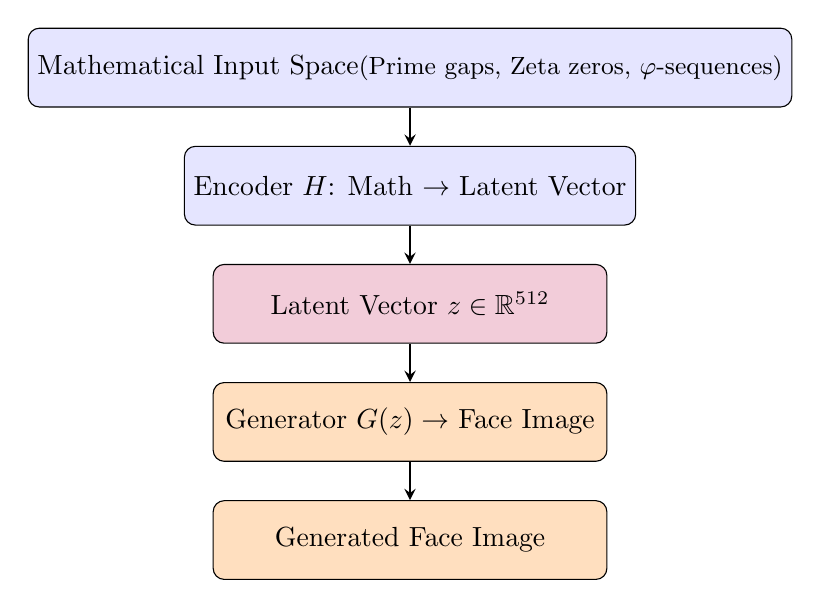
\begin{tikzpicture}[node distance=1.5cm]
\tikzstyle{block} = [rectangle, rounded corners, minimum width=5cm, minimum height=1cm,
                    text centered, draw=black, fill=blue!10]
\tikzstyle{latent} = [block, fill=purple!20]
\tikzstyle{imagegen} = [block, fill=orange!25]
\tikzstyle{arrow} = [thick,->,>=stealth]
\node (math) [block] {Mathematical Input Space\\ \small{(Prime gaps, Zeta zeros, $\phiGR$-sequences)}};
\node (encoder) [block, below of=math] {Encoder $H$: Math $\rightarrow$ Latent Vector};
\node (z) [latent, below of=encoder] {Latent Vector $z \in \RR^{512}$};
\node (generator) [imagegen, below of=z] {Generator $G(z) \rightarrow$ Face Image};
\node (output) [imagegen, below of=generator] {Generated Face Image};
\draw [arrow] (math) -- (encoder);
\draw [arrow] (encoder) -- (z);
\draw [arrow] (z) -- (generator);
\draw [arrow] (generator) -- (output);
\end{tikzpicture}
\end{center}
% ==========================================================
\section{$\phi$-SDE Latent Refinement Layer}
% ==========================================================
\subsection{Forward SDE}
Let $\phiGR=(1+\sqrt5)/2$. Define the forward SDE on $\cZ$:
\begin{align}
d\mathbf{z}_t &= f(\mathbf{z}_t,t)\,dt + g(t)\,d\omega_t,\\
g(t) &= \gamma\sqrt{1-\phiGR^{-2t}},\\
f(\mathbf{z}_t,t) &= -\phiGR^{-t}\big(\mathbf{z}_t-\Pi_{\mathrm{QAM}}(\mathbf{z}_t)\big),
\end{align}
where $\Pi_{\mathrm{QAM}}$ is a projection onto a chosen ``quantum-arithmetic manifold''
(or a practical substitute such as an identity/anchor manifold).
\begin{remark}
For an MVP, $\Pi_{\mathrm{QAM}}$ may be implemented as an identity-preserving projector
(e.g., toward a HELEN anchor latent), then refined later.
\end{remark}
\subsection{Reverse SDE (sampling / correction)}
The reverse-time dynamics are:
\begin{equation}
d\mathbf{z}_t =
\left[f(\mathbf{z}_t,t)-g(t)^2\nabla_{\mathbf{z}}\log p_t(\mathbf{z}_t)\right]dt
+ g(t)\,d\bar{\omega}_t,
\end{equation}
where a score network $s_\theta(\mathbf{z},t)\approx \nabla_{\mathbf{z}}\log p_t(\mathbf{z})$
is trained via denoising score matching.
\subsection{Minimal implementation surface}
The minimal code API surface corresponds to:
\texttt{diffusion\_schedule(t)}, \texttt{phi\_drift(z,t)}, \texttt{PhiScoreNet},
\texttt{forward\_sde}, \texttt{reverse\_sde}. (Documented as the minimal framework components.)
% ==========================================================
\section{Identity Preservation and Round-Trip Criteria}
% ==========================================================
\subsection{Identity preservation functional}
Define:
\[
\IP(\delta)=\sup_{d_{\cM}(m_1,m_2)<\delta}\ \big\|G(H(m_1))-G(H(m_2))\big\|_{\cI}.
\]
Operational thresholds:
\begin{itemize}
\item $\delta\le 0.1$: preserved
\item $0.1<\delta\le 0.3$: slight shift
\item $0.3<\delta\le 0.5$: major change
\item $\delta>0.5$: identity break
\end{itemize}
\subsection{Round-trip invariants}
We enforce (at minimum) the round-trip constraint:
\[
H^{-1}\!\left(E\!\left(G(H(m))\right)\right)=m,
\]
up to declared tolerances (exact for discrete objects; approximate for continuous parameters).
% ==========================================================
\section{Optional: Q$\Phi$-SoftPrompt Editing (Controlled Attribute Edits)}
% ==========================================================
\begin{definition}[Q$\phiGR$ softprompt]
Given a latent $z\in\cZ$, define an edit operator
\[
Q_{\phiGR}(z)=z+\sum_{k=1}^m \alpha_k(\phiGR)\,\mathcal{B}_k(z),
\]
where $\mathcal{B}_k$ are basis transforms derived from prime/zeta/fractal motifs.
\end{definition}
\begin{definition}[Prime-driven Hamiltonian edit]
Define
\[
H_{\phiGR}=\sum_{k=1}^m \phi_k\,|u_k\rangle\langle u_k|,
\quad\text{with}\quad u_k[i]=\mathrm{bit}_i(p_k),
\]
and a small-step update $z' = z + \Delta t\, H_{\phiGR} z$.
This module is used only for \emph{controlled} edits (pose/style/lighting) while maintaining identity gates.
\end{definition}
% ==========================================================
\section{Pre-Registered Gates and Reproducibility Protocol}
% ==========================================================
\subsection{Pre-registered computational gates}
\begin{proposition}[Falsifiable gates]
The assistant uses pre-registered pass/fail gates:
\begin{itemize}
\item \textbf{Gate S (Scattering):} permutation test with BH-FDR at $\alpha=0.05$;
\textbf{pass} if discoveries exceed the 99th percentile of the null.
\item \textbf{Gate A (AEON Trend):} Mann--Kendall trend test (with Theil--Sen slope) on a score series;
\textbf{pass} if a statistically significant negative trend is detected (e.g.\ $\tau<0$, $p<0.01$,
and 95\% CI of slope strictly negative).
\end{itemize}
\end{proposition}
\subsection{Reproducibility contract (artifacts + one-command rebuild)}
\begin{proposition}[Reproducibility protocol]
Each run MUST emit an artifact bundle:
\begin{itemize}
\item YAML/JSON config snapshot (including latent dimension, model identifiers, seed)
\item hashed inputs (math object serialization and/or reference images)
\item outputs: images + latents $(z_0,z_T,\hat z_0)$ + gate metrics
\item a verification script that replays the run and reproduces figures/tables
\end{itemize}
and a containerized environment with a Makefile target that regenerates results in one command.
\end{proposition}
\section{Assistant Runtime Interface (Operational Protocol)}
\begin{enumerate}[leftmargin=*]
\item \textbf{Ingest/Anchor:} build HELEN identity anchors (face embeddings; optional 3D constraints).
\item \textbf{Math$\to$Face:} $m\mapsto z_0=H(m)\mapsto \hat z_0$ via $\phi$-SDE refine $\mapsto \hat I=G(\hat z_0)$.
\item \textbf{Face$\to$Math:} $I\mapsto z=E(I)\mapsto \hat m=H^{-1}(z)$.
\item \textbf{Validate:} compute round-trip + identity gates; return PASS/FAIL with metrics.
\item \textbf{Edit (optional):} apply Q$\phiGR$ edits, then re-run gates.
\end{enumerate}
\end{document}
